\documentclass[a4paper,10pt]{scrartcl} % Die documentclass darf in keiner Latex-Datei fehlen, wenn die Datei allein ein Dokument erstellen soll. Es gibt allerdings die Möglichkeit andere Dateien, die Latex-Code enthalten in ein bestehendes Dokument einzubinden. Das geht mit "\include{anderesDokument}" oder "\input{andresDokument}" und ist besonders bei laaaaaaangen Dokumenten praktisch.
\usepackage[utf8]{inputenc}
\usepackage[german]{babel}
%\usepackage[T1]{fontenc}        % Erweiterte Textcodirung (z.B a" -> ä)
\usepackage{hyperref,url}       % Hyperlinks im pdf
\usepackage[all]{hypcap}        % Verhaltenskorrektur für hyperref
\usepackage{amssymb,amsmath}    % Schöne Formeln (AMS = American Mathematical Society)
\usepackage{graphicx}           % Bilder und Seitenränder
\usepackage{natbib}		        % Bessere Bibliographie
%\bibliographystyle{dinat}       % Literaturverzeichnis nach DIN1505
%\usepackage{unicode-math}
\usepackage{caption}
\usepackage{pdfpages}



\subject{Fortgeschrittenenpraktikum 1, Universit\"at Innsbruck}
\title{Elektronenspinresonanz}
\author{Gruppe T,Simon Hangl\footnote{\href{mailto:simon.hangl@uibk.ac.at}Simon.Hangl@uibk.ac.at}, Georg Zagler\footnote{\href{mailto:georg.zagler@student.uibk.ac.at}Georg.Zagler@student.uibk.ac.at}}
\date{Innsbruck, \today}



\begin{document}
\maketitle
\newpage{}
\tableofcontents{}
\newpage{}

\begin{abstract}
Der Versuch über die Elektronenspinresonanz gibt Aufschluss darüber, wie sich das Eigendrehmoment eines Elektrons verhält. Durch das Studium der Theorie ist es möglich das Verhalten eines Drehmomentes unter dem Einfluss eines externen Feldes vorherzusagen. Dadurch lässt sich das intrinsische Drehmoment (Spin) eines Elektrons durch das Anlegen und Kontrollieren eines Magnetfeldes bestimmen und umgekehrt die Stärke eines Magnetfeldes bestimmen, wenn man Kenntnis über das qualitative Verhalten eines Spins hat.
\end{abstract}
\section{Einleitung}
\label{sec:einleitung}
Der Versuch von Stern und Gerlach demonstrierte, dass Teilchen ein intrinsisches magnetisches Moment besitzen können\cite{Schwabl}. Dieses Moment rührt vom Elektronenspin her. In seiner Beschreibung unterliegt der Spin derselben Algebra wie der Drehimpuls. Beschreibt man jedoch das magnetische Moment des Elektronenspins analog zum Bahndrehimpuls des Elektrons, so erhält man ein Ergebnis, welches um eine Konstante $g_S$ zu klein ist. Dieser klassisch nicht erwartete Landé-Faktor wurde in diesem Versuch ermittelt. Im zweiten Teil des Versuches verwendeten wir den bestimmten $g$-Faktor um umgekehrt Rückschlüsse auf die Stärke des Magnetfeldes zu ziehen und die magnetische Flussdichte eines Paramagneten zu bestimmen.\\
In dem Versuch verwendeten wir einen Aufbau, wo homogene und inhomogene Magnetfelder überlagert werden, um die Spin-Eigenschaft eines Materials zu prüfen. Ähnliche Methoden werden im medizinischen Bereich bei der Magnetresonanztomographie verwendet, um Rückschlüsse auf die Zusammensetzung eines Gewebes oder Organes zu ziehen, ohne dieses zu sezieren.

\section{Theorie und Grundlagen}
\label{sec:theorie}
\subsection{Helmholtz-Spule}
\label{subsec:helmholtz}
\begin{minipage}[t]{0.5\textwidth}
	Eine Helmholtz-Spule besteht aus zwei parallel ausgerichteten Spulen mit gleichläufigem Strom. Bei einer solchen Symmetrie wird aus dem Biot-Savart-Gesetz
	\begin{equation}
	\label{eqn:biot-savart}
	d\mathbf{B(r)} = \frac{\mu _0}{4 \pi} I d\mathbf{l} \wedge \frac{\mathbf{r - r_0}}{(\mathbf{r - r_0})^3}
	\end{equation}
	\begin{equation}
	\label{eqn:helmholtz}
	B(R/2) = \mu _0 \frac{8 I}{\sqrt{125} R}
	\end{equation}
\end{minipage}
\hfill
\begin{minipage}[t]{0.55\textwidth}
\label{fig:helmholtz}
  \raisebox{\dimexpr-\totalheight+\ht\strutbox\relax}{%
	\includegraphics[width=0.85\textwidth]{Bilder/helmholtz.png}
  }
\captionof{figure}{Feldverlauf in einer Helmholtzspule (Bild entnommen aus: abi-physik.de).}
\end{minipage}
\\
Wo Gleichung (\ref{eqn:helmholtz}) ein homogenes Feld entlang einer Richtung in der Mitte des Spulenpaares beschreibt, wie in Abbildung.
\subsection{Paramagnetische Substanzen}
Eine paramagnetische Substanz zeichnet sich dadurch aus, dass es ein externes magnetisches Feld im Inneren verstärkt. Es besitzt ein ungepaartes Elektron.
Ein ungepaartes Elektron besitzt ein magnetisches Moment $\boldsymbol{\mu}_S = g\mu_B\mathbf{S}$. Dieses ist parallet zum Elektronenspin $\boldsymbol{\mu}_S$ und abhängig vom Landé-Faktor g und vom Bohrschen Magneton $\mu_B$. In einem externen magnetischen Feld $B$ ändert sich die Energie des Elektrons gemäß $\Delta U = -\mu B$.
Eine Zustandsänderung des Spins $|\chi>$ vom Zustand $|s_z=-1/2>_{\chi}$ in den Zustand $|s_z=1/2>_{\chi}$ erfordert die Wechselwirkung mit einem elektromagnetischen Strahlungsfeld der Energie 
\begin{equation}
\label{eqn:dipol}
E = \hbar \omega = g\mu_BB
\end{equation}
über magnetische Dipolstrahlung \citep{Anleitung}\footnote{Die Anleitung zum Versuch wird an verschiedenen Stellen zur Beschreibung der Theorie verwendet.}.
\subsection{Physikalische Prozesse im Versuch}
\label{subsec:prozesse}
In diesem Versuch haben wir eine Paramagneische Substanz verwendet. Ein Magnetfeld wird in $z$-Richtung eingeschalten. Der Spin des ungepaarten Elektrons der Substanz führt eine Präzessionsbewegung um die $z$-Achse aus. Dies liegt daran, dass der Spin quantisiert ist und seine Ausrichtung nicht ausschließlich in eine Raumachse erfolgen kann. Es ergibt sich ein Drehmoment
\begin{equation}
\label{eqn:drehmoment}
\vec{M} = \vec{\mu} \wedge \vec{B} = const. \cdot \vec{D} \wedge \vec{B}
\end{equation}
wegen der Wirkung des externen Magnetfeldes auf den Eigendrehimpuls (Spin). Der Spin rotiert dabei mit der $Larmor$-Frequenz $\omega _L = const. \cdot \vec B$ um die $z$-Achse. Die $Larmor$-Frequenz entspricht genau der Frequenz $\omega$ aus Gleichung (\ref{eqn:dipol}).\\
\textbf{Spin-Flip}\\
Schaltet man ein zusätzliches Magnetfeld $\vec{B}$ mit wechselnder Flussdichte so ein, dass es periodisch in der $x$-$y$-Ebene mit der Winkelgeschwindigkeit $\omega = \omega _L$ oszilliert, so wirkt es für den mit $\omega _L$ um die $z$-Achse rotierenden Spin wie ein konstantes Magnetfeld.
\begin{equation}
\label{eqn:hochfrequenz Magnetfeld}
\vec{B}_{HF}(t) = \left( \begin{array}{c}
B_{HF} \cos( \omega t)\\
B_{HF} \cos( \omega t)\\
0\\
\end{array} \right)
\end{equation}
Dieses für den Spin konstante Magnetfeld übt auf den Spin, wie in Gleichung (\ref{eqn:drehmoment}) beschrieben, ein Drehmoment aus. Dieses Drehmoment dreht den Eigendrehimpuls (Spin) je nach Orientierung nach unten oder nach oben. Um seine Lage zu ändern muss der Spin Energie aus dem mitrotierenden Magnetfeld aufnehmen, da die verschiedenen Zustände des Spins im externen Magnetfeld verschiedene Energien besitzen. In unserem Versuchsaufbau wurde das mitbewegende Magnetfeld durch eine langgezogene Spule in einem Schwingkreis erzeugt. Da der Strom proportional zum erzeugten Magnetfeld ist, konnte man den Abfall des Magnetfeldes messen.
\section{Aufbau}
\label{sec:aufbau}
\begin{minipage}[t]{0.5\textwidth}
	Der Versuch wurde aufgebaut aus:
	\begin{itemize}
	\item Probenampulle mit DPPH
	\item Helmholtz-Spulenpaar (d = 30cm, N = 124 Windungen)
	\item Spartransformator
	\item Stromgeregeltes Labornetzgerät für Gleichstrom
	\item Hilfsspulen
	\item Schwingkreis mit langgezogener Spule
	\item Multimeter
	\item Oszilloskop
	\item Magnetfuß
	\item Stahllineal
	\item Kabel
	\end{itemize}
\end{minipage}
\hfill
\begin{minipage}[t]{0.4\textwidth}
\label{fig:Aufbau}
  \raisebox{\dimexpr-\totalheight+\ht\strutbox\relax}{%
	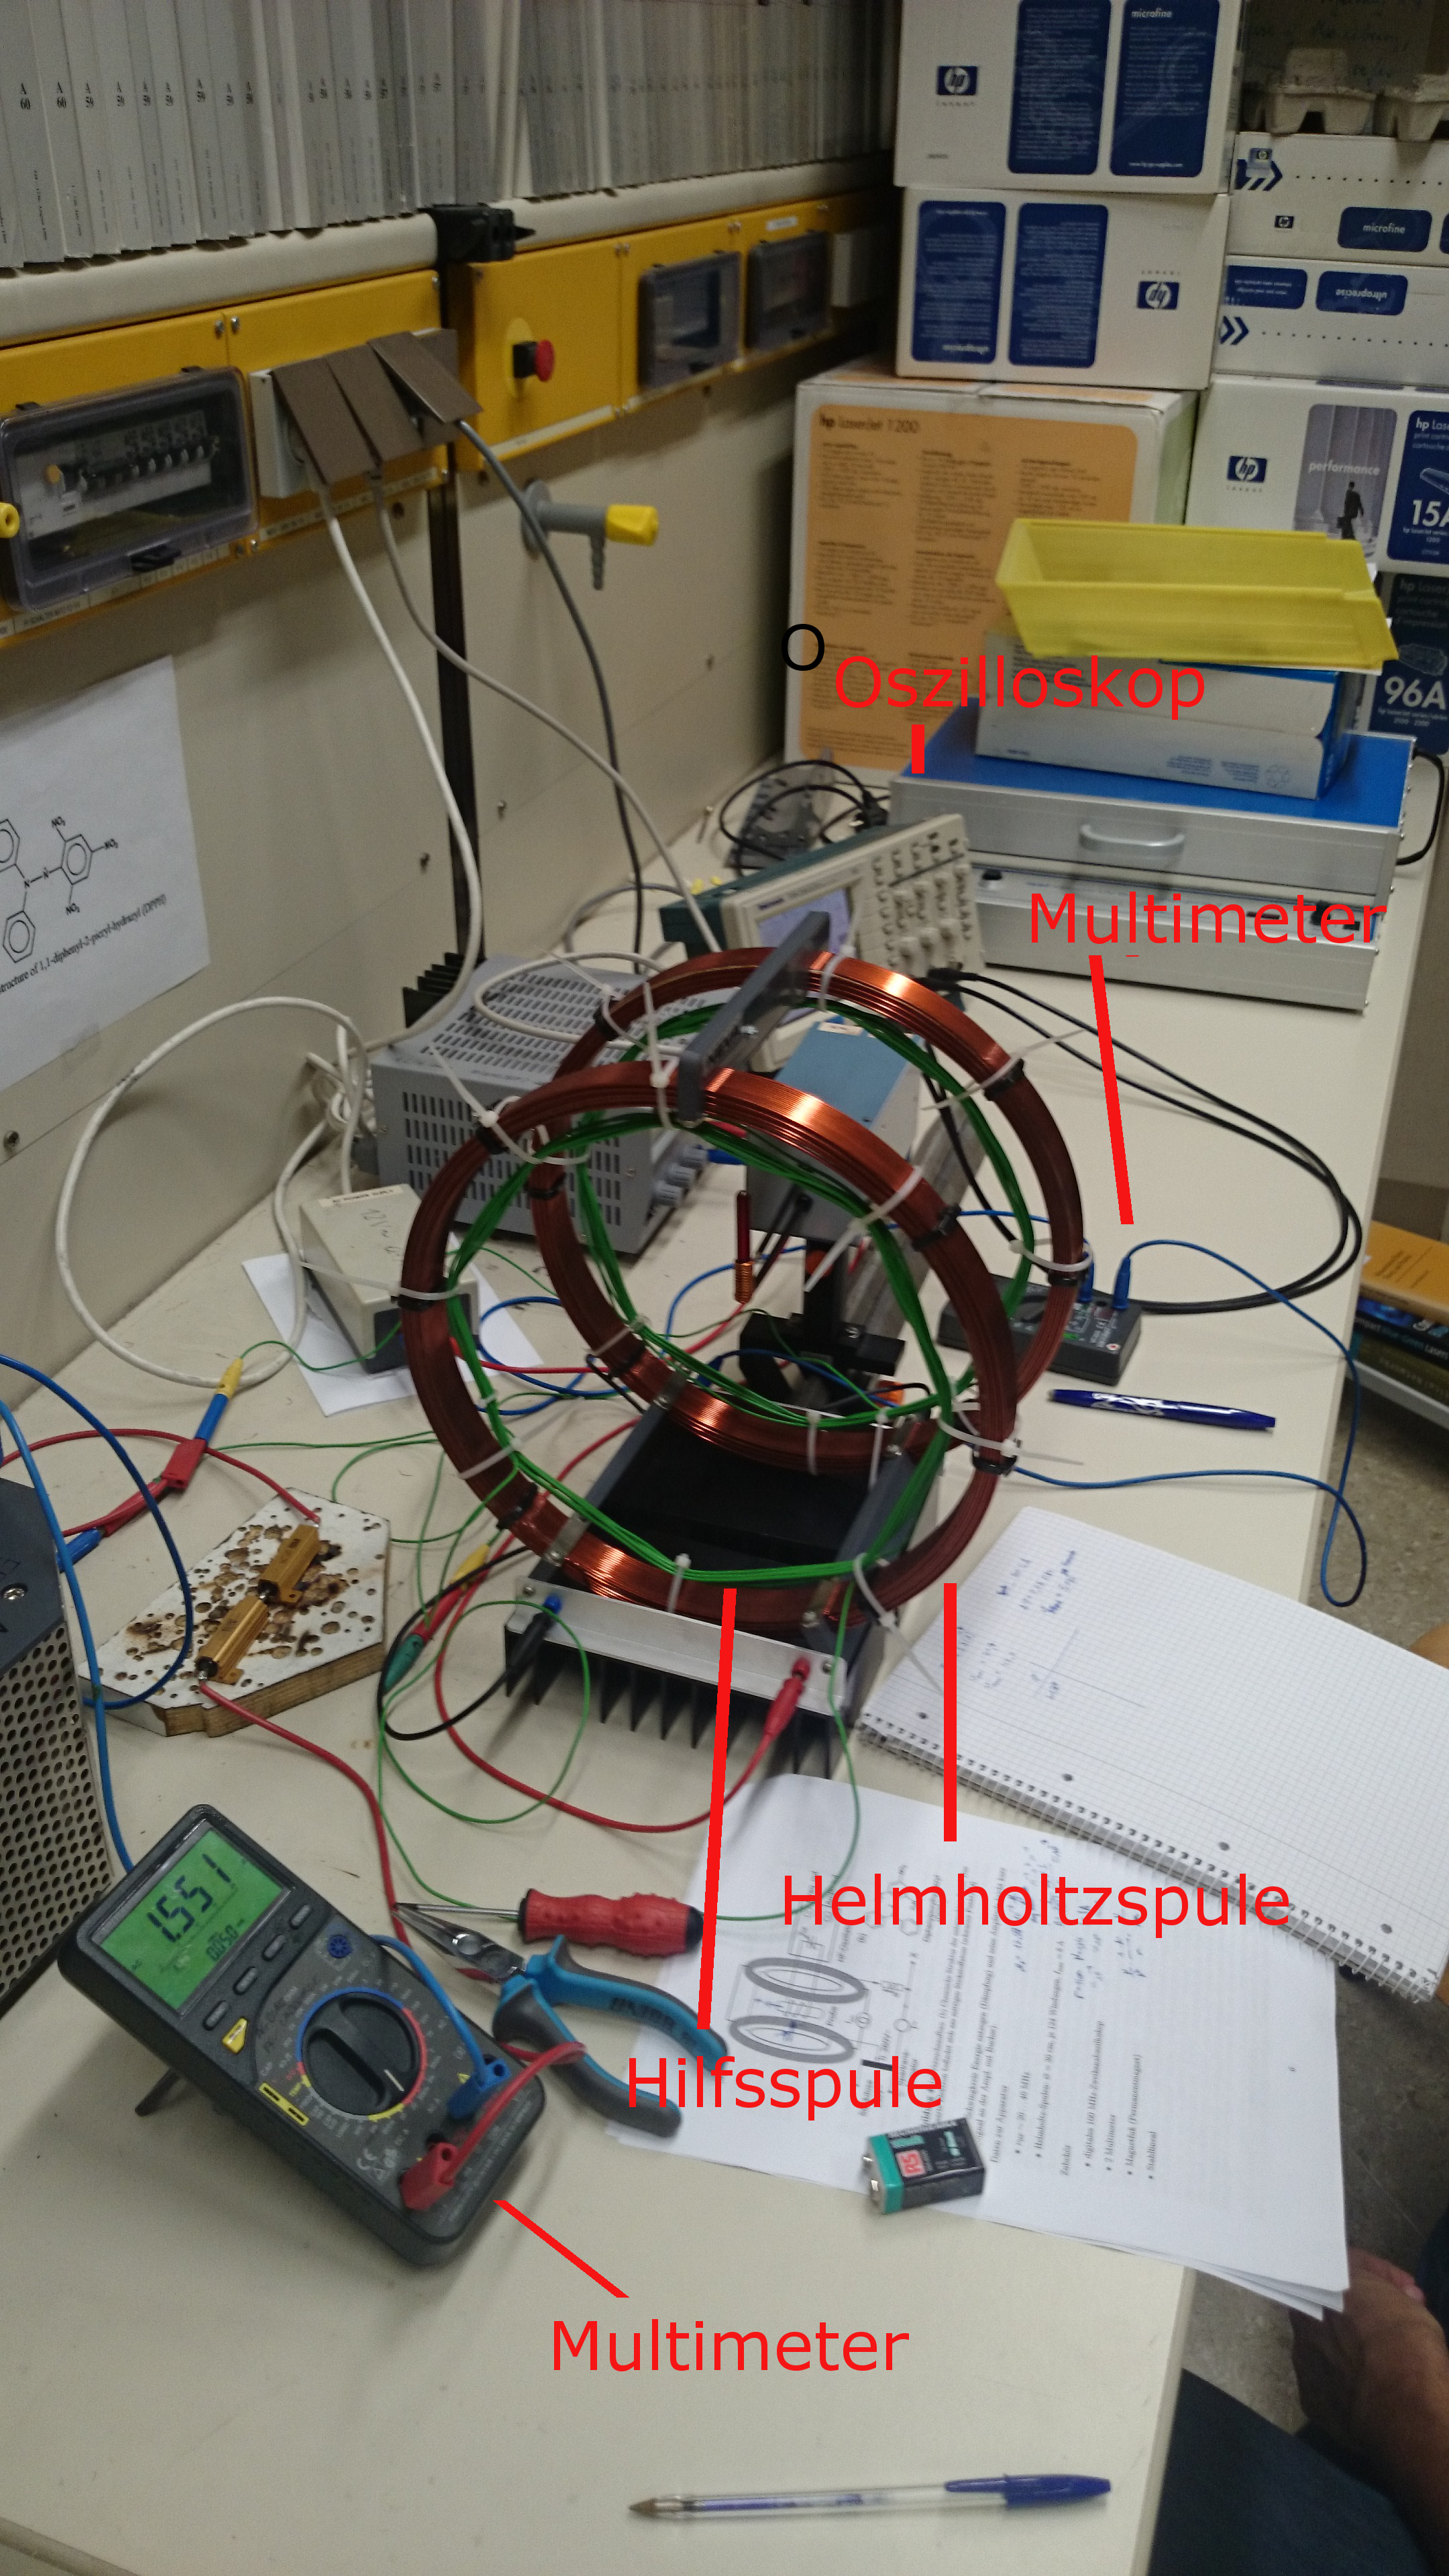
\includegraphics[width=0.9\textwidth]{Bilder/spin/Aufbau.png}
  }
\captionof{figure}{Versuchsaufbau}
\end{minipage}
\\
Das Helmholtz-Spulenpaar wurde mit dem Labornetzgerät betrieben. Das Labornetzgerät musste wegen der Gleichspannung richtig gepolt mit der Steckdose verbunden werden. Der Spulenstrom $I_{DC}$ wurde mit einem Multimeter gemessen. Die Hilfsspulen wurden innen um beide Helmholtz-Spulen gewickelt. Sie modulierte das homogene Magnetfeld innerhalb der Spule mit einer Frequenz von 50 Hz sodass die Resonanzfrequenz leichter gefunden werden kann. Die Ampulle mit der Diphenylpicrylhydracyl-Probe (DPPH; ist paramagnetisch) wurde in die Spule des Hochfrequenz-Oszillators gesteckt. Diese befand sich mittig zwischen beiden Helmholtz-Spulen. Mit einem Multimeter wurde der Strom im Hochfrequenz-Schwingkreis gemessen. Die Frequenz  und der Strom des Schwingkreises wurden am Oszillator dargestellt.

\section{Durchführung}
\label{sec:durchfuehrung}
\subsection{Bestimmung des g-Faktors}
\label{subsec:g-Faktor}
Im ersten Teil des Versuches verwendeten wir verscheidene Stromstärken der Helmholtzspule um den $g$-Faktor zu bestimmen. Dazu musste zu jeder Stromstärke die entsprechende Resonanzfrequenz des Schwingkreises gefunden werden. Um die Resonanzfrequenz des Schwingkreises, bei dem es einen Spin-Flip bewirkt, zu finden, wurde die Amplitude des Schwingkreises im Oszillator betrachtet und die Frequenz so lange verändert, bis man einen Einbruch der Amplitude beobachtete. In der Feinjustage wurde die Frequnz so verändert, dass doppelt so viele gleichmä\ss ige Einbrüche zu beobachten waren. Doppelt so viele Einbrüche bedeuten hierbei, dass das Wechselfeld der Hilfsspule zusammen mit dem konstanten Feld der Helmholtz-Spule ein Feld $B = B_{Helmholtz} + B_{Hilf}$ erzeugt, zu welchem der Schwingkreis mit der Frequenz $\omega$ resonant ist. Gleichmä\ss ige Einbrüche bedeuten, dass die Abstände zwischen den zu $\omega$ resonanten $B$-Felder ebenfalls gleichmä\ss ig sind und somit die Resonanzfrequenz genau bei dem Magnetfeld $B_{ges}(t) = B_{Helmholtz}$ auftritt (vgl. Abbildung (\ref{fig:Resonanz}).
\begin{figure}
\label{fig:Resonanz}
\includegraphics[width=\textwidth]{Bilder/sinus.png}
\caption{Gesamtmagnetfeld in $z$-Richtung aus überlagerung der Felder der Helmholtzspule (hellblaues Kästchen) mit dem wechselnden Hilfsfeld (Sinusförmig) und die Erfüllung der Resonanzbedingung beim Schnitt mit der Geraden.}
\end{figure}
Am Oszillator wurde dann die Resonanzfrequenz gemessen.
\subsection{Feldstärkebestimmung}
\label{subsec:Feldstaerkebestimmung}
Im zweiten Teil des Versuches wurde der selbe Aufbau verwendet, jedoch wurde ein Permanentmagnet, welcher ein zusätzliches magnetisches Feld erzeugt, zwischen die Helmholtz-Spulen gegeben. Dadurch wollen wir mit dem Wissen über den Effekt eines zusätzlichen Magnetfeldes auf die Resonanz, die Stärke des Magneten bestimmen. Der Schwingkreis wurde auf eine feste Frequenz $\nu _{HF} = 29.9(1)$ fixiert. Dann wurde der Magnet in vier Positionen jeweils parallel und senkrecht zum Magnetfeld der Helmholtz-Spulen ausgerichtet und der für die Resonanz notwendige Spulenstrom $I_{SP}$ gemessen.
\section{Auswertung}
\label{sec:auswertung}
\subsection{g-Faktor}
\label{subsec:g-Faktor}
Aus dem Kapitel (\ref{sec:theorie}) geht hervor, dass das durch die Helmholtz-Spule erzeugte Magnetfeld $\vec{B}$ proportional zum Spulenstrom ist und dass die Frequenz des Schwingkreises der $Larmor$-Frequenz $\omega _L$ entsprechen muss, um einen Spin-Flip zu erreichen (vgl. Unterabschnitt (\ref{subsec:prozesse}). Im resonanten Fall erhält man daher die Relation
\begin{equation}
\label{eqn:Auswertung-g-faktor}
\omega _{Schwingkreis} = \omega _L = \frac{g \mu _B B}{\hbar} =  \frac{8 \mu _0 g \mu _B I_{Helmholtz}}{\sqrt{125} R \hbar}
\end{equation}
\begin{figure}
\label{fig:g-faktor-slope}
\includegraphics[width=\textwidth]{Daten/g-faktor.png}
\caption{Darstellung der Resonanzfrequenz f in Abhängigkeit des Helmholtz-Spulen-Stroms I.}
\end{figure}
In Abbildung (\ref{fig:g-faktor-slope}) wurden die beiden Messgrö\ss en $f = \omega _{HF} = \omega _L$ und $I_{Helmholtz}$ geplottet. Die Steigung des linearen Fits beträgt $A = 2.136 \frac{Mhz}{A}$ und der Offset $B = 0.04 Mhz$.\\
In Abbildung (\ref{fig:wertetabelle}) werden die Daten und die daraus berechneten g-Faktoren dargestellt. NIST\footnote{http://physics.nist.gov/cgi-bin/cuu/Value?gem} gibt den Wert des g-Faktors mit $g = -2.002 319 304 361 53(53)$ an.\\
Wir haben den $g$-Faktor aus dem Fit mit $g = 2.0526(4)$ und aus dem Mittelwert der Messwerte mit $g = 2.079(11)$ berechnet. Zur Berechnung des Fehlers haben wir Gauss-Fehlerfortpflanzung verwendet und angenommen, dass die einzigen Fehlerquellen das Oszilloskop und die genaue Bestimmung des Spulenstroms mit dem Amperemeter sind.\\
Der Offset wird gemä\ss der Herleitung nicht erwartet, jedoch wird darin angenommen, dass das magnetische Feld nur durch die Spulen erzeugt wird. Weitere elektrische Felder, z.B. das der Erde, schlecht isolierter elektrischer Leitungen in der Umgebung, oder vonFerromagneten in der Umgebung, kann sich mit dem Feld der Spulen überlagern und so die Ergebnisse verfälschen.

\subsection{Feldstärkebestimmung eines Permanentmagneten}
\label{subsec:Auswertung-Feldstaerkebestimmung}
In der Spule addieren sich die magnetischen Felder der Magneten und der Spule vektoriell zu einem Magnetischen Feld $\vec{B}_{res} = \vec{B}_HS + \vec{B}_{Magnet}$. Wir nehmen in unserer Berechnung an, dass der Magnet zentral unter der Probe steht, sodass dessen Magnetfeld keine Komponente in der vertikale Richtung (wird ab hier als $z$ bezeichnet) besitzt. Es ergibt sich
\begin{equation}
|\vec{B}_{ges}| = | \left( \begin{array}{c}
B_{HS}\\
0\\
0\\
\end{array} \right) + \left( \begin{array}{c}
B_{Magnet} \cdot \cos (\alpha)\\
B_{Magnet} \cdot \sin (\alpha)\\
0\\
\end{array} \right)
| = \sqrt{(B_{HS}+ B_{Magnet}\cos(\alpha))^2 + (B_{Magnet}\sin(\alpha))^2}
\end{equation}
Mit der Mitternachtsformel ergibt sich:
\begin{equation}
\label{eqn:Mitternachtsformel}
B_M = -B_{HS}\cos (\alpha) \pm \sqrt{B_{HS}^2 \cos ^2(\alpha) - (B_{HS}^2 - B_{ges}^2)}
\end{equation}
woraus man durch Umstellen erhält:
\begin{equation}
\label{eqn:Auswertung2}
B_M = -B_{HS} \cos (\alpha) \pm \sqrt{B^2_{HS} \cos ^2 (\alpha) + B^2_{ges} - B^2_{HS}}
\end{equation}
Wir gehen davon aus, dass der Magnet wegen einer fehlenden Referenz zum Festlegen des Winkels eine Ungenauigkeit von $\Delta \alpha = 7^\circ$ besitzt. Der Fehler des beim ablesen von der Spule wurde wieder mit 0.02 A abgeschätzt. Der Gesamtfehler wurde mit Gauss-Fehlerfortpflanzung in Excel berechnet.

\newpage
\section{Appendix}
\label{sec:appendix}
\textbf{Rechnungen}\\
Aus den gemessenen Daten (Abbildung (\ref{fig:wertetabelle})).
\begin{equation}
\label{eqn:g-Fehler1}
g = \frac{\sqrt{125} R \hbar}{8 \mu _0 \mu _B I_{SP}} \nu _HF \; \Rightarrow \; (\Delta g)^2 = (\frac{\sqrt{125} R \hbar}{8 \mu _0 \mu _B I_{SP}})^2( (\Delta \nu _{HF})^2 + (\frac{\Delta I_{SP}}{I_{SP}})^2)
\end{equation}
Aus dem Fit der Daten mit Steigung k.
\begin{equation}
\label{eqn:g-Fehler2}
g = \frac{\sqrt{125} R \hbar}{8 \mu _0 \mu _B} \cdot 10^6 k \; \Rightarrow \; (\Delta g)^2 = (\frac{\sqrt{125} R \hbar}{8 \mu _0 \mu _B})^2 \cdot (10^6 \Delta k)^2
\end{equation}
\begin{figure}
\label{fig:wertetabelle}
\begin{minipage}{0.65\textwidth}
	\includegraphics[width=\textwidth]{Daten/Tabelle.pdf}
\end{minipage}
\begin{minipage}{0.65\textwidth}
\includegraphics[width=\textwidth]{Daten/Tabelle2.pdf}
\end{minipage}
\caption{Messwerte.}
\end{figure}
\newpage
\bibliographystyle{plain}
\bibliography{Elektronenspinresonanz}
\end{document}